\documentclass[tikz, border=3pt]{standalone}

\usepackage{tikz}
\usepackage{pgfplots}

\begin{document}
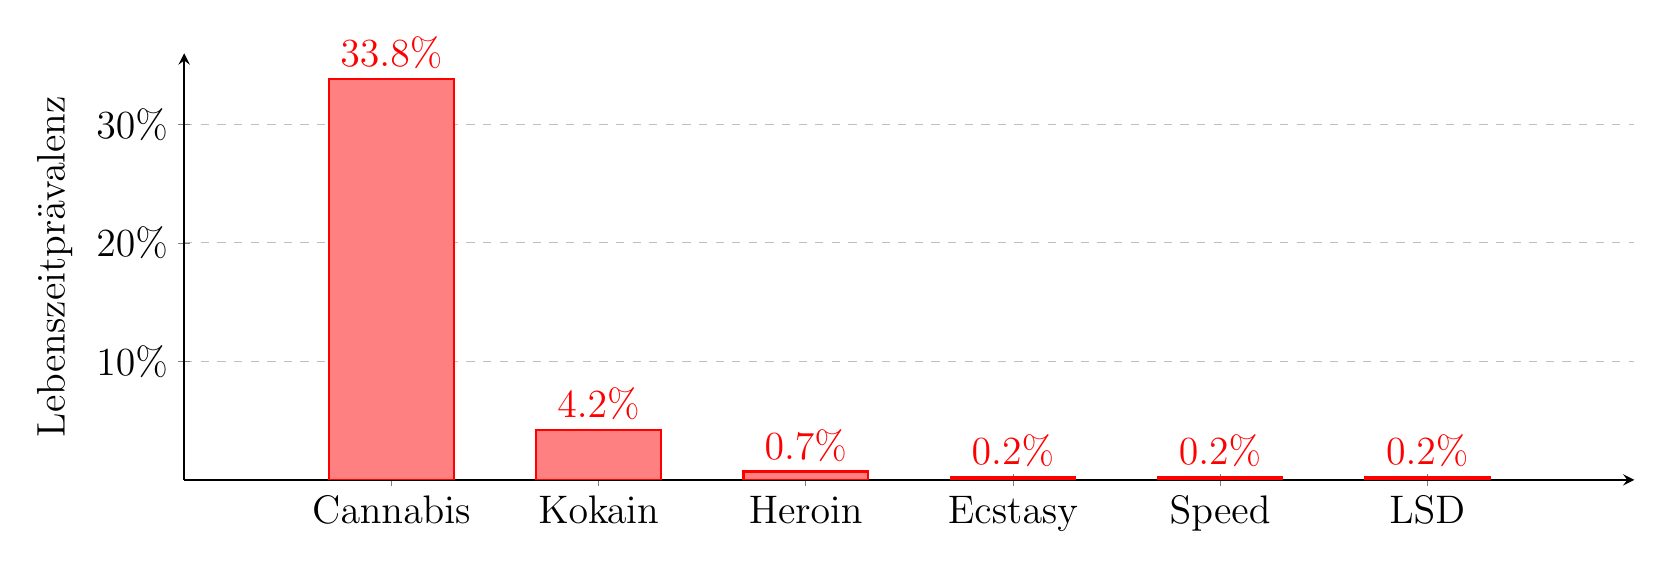
\begin{tikzpicture}

\begin{axis}[
	thick,
	ylabel = {\Large Lebenszeitprävalenz},
	xmin=0, xmax=7,
	ymin=0, ymax=36,
	width=20cm,
	height=7cm,
    xtick = {1,2,3,4,5,6},
	xticklabels={
		\Large Cannabis,
		\Large Kokain,
		\Large Heroin,
		\Large Ecstasy,
		\Large Speed,
		\Large LSD
	},
	yticklabel={\Large\pgfmathprintnumber\tick\%},
	axis lines=middle,
    ymajorgrids,
    grid style={dashed},   
    x label style={at={(axis description cs:0.5,-0.15)},anchor=north},
    y label style={at={(axis description cs:-0.07,.5)},rotate=90,anchor=south},
]


	
% Cannabis
\addplot[
	ybar, 
	color=red,
	fill=red!50!,
	bar width=45pt,
	nodes near coords=\Large\pgfmathprintnumber{\pgfplotspointmeta}\%,
] coordinates {
	(1, 33.8)
	(2, 4.2)
	(3, 0.7)
	(4, 0.2)
	(5, 0.2)
	(6, 0.2)
};

\end{axis}

\end{tikzpicture}
\end{document}